% This must be in the first 5 lines to tell arXiv to use pdfLaTeX, which is strongly recommended.
\pdfoutput=1
% In particular, the hyperref package requires pdfLaTeX in order to break URLs across lines.

\documentclass[11pt]{article}

% Remove the "guidelines" option to generate the final version.
%\usepackage[guidelines]{nlpreport} % show guidelines
\usepackage[]{nlpreport} % hide guidelines

% Standard package includes
\usepackage{times}
\usepackage{latexsym}

% For proper rendering and hyphenation of words containing Latin characters (including in bib files)
\usepackage[T1]{fontenc}
% For Vietnamese characters
% \usepackage[T5]{fontenc}
% See https://www.latex-project.org/help/documentation/encguide.pdf for other character sets

% This assumes your files are encoded as UTF8
\usepackage[utf8]{inputenc}

% This is not strictly necessary, and may be commented out,
% but it will improve the layout of the manuscript,
% and will typically save some space.
\usepackage{microtype}
\usepackage{graphicx}
\usepackage{hyperref}
\usepackage{amsmath}
\usepackage{mathtools}
\usepackage{multirow}
\usepackage{listings}
\usepackage{xcolor}
\usepackage{booktabs} % for tables

% THE pdfinfo Title AND Author ARE NOT NECESSARY, THEY ARE METADATA FOR THE FINAL PDF FILE
\hypersetup{pdfinfo={
Title={Removing Sensitive Sentences from Italian Expert Appraisals},
Author={Klein Tahiraj}
}}
%\setcounter{secnumdepth}{0}  
 \begin{document}
%
\title{Removing Sensitive Sentences from Italian Expert Appraisals:\\ Distillation, Shortcuts and Counterfactual Repair\\
\explanation{\rm Substitute $\uparrow$ this title $\uparrow$ with your project's title\\ \smallskip}
% subtitle:
\large 
3-cfu Project Work in Natural Language Processing
}
\author{Klein Tahiraj\\
Master's Degree in Artificial Intelligence, University of Bologna\\
klein.tahiraj@studio.unibo.it
}
\maketitle

\attention{DO NOT MODIFY THIS TEMPLATE - EXCEPT, OF COURSE FOR TITLE AND AUTHOR INFORMATION.\\ IN THE FINAL VERSION, IN THE \LaTeX\ SOURCE REMOVE THE \texttt{guidelines} OPTION FROM  \texttt{$\backslash$usepackage[guidelines]\{nlpreport\}}.
}

\begin{abstract}
%\begin{quote}

% write your abstract here
Real-estate enforcement proceedings require expert appraisals, which often mention the health, criminal history, minors and family circumstances of the people involved, and the GDPR requires stripping them before sharing these documents. In this work, we train a cheap and fast model that removes sentences with sensitive facts about a living person. Without an annotated corpus, we distil the labels of LLM annotators under a fixed two-gate policy, verified on a human-labelled sample, into an mDeBERTa classifier, adding counterfactual pairs and a pairwise margin loss. The selected variant removes 371 of 372 sensitive sentences in unseen appraisals while deleting about 5\% of the harmless ones, far above entity-based tools and a zero-shot 12B LLM, and unlike the first model it keeps most negated sentences, which must not be removed.

\explanation{
The abstract is very brief summary of your report. Try to keep it no longer than 15-20 lines at most. Write your objective, your approach, and your main observations (what are the findings that make this report worthwhile reading?)}

%\end{quote}
\end{abstract}

\attention{\textcolor{red}{NOTICE: THIS REPORT'S LENGTH MUST NOT EXCEED \textbf{8 PAGES}  PLUS AI REPORT, LINKS, REFERENCES AND APPENDICES.\\ 
THIS MEANS THAT YOU CANNOT FILL ALL SECTIONS TO MAXIMUM LENGTH. IT ALSO MEANS THAT, QUITE POSSIBLY, YOU WILL HAVE TO LEAVE OUT OF THE REPORT PART OF THE WORK YOU HAVE DONE OR OBSERVATIONS YOU HAVE. THIS IS NORMAL: THE REPORT SHOULD EMPHASIZE WHAT IS MOST SIGNIFICANT, NOTEWORTHY, AND REFER TO THE NOTEBOOK FOR ANYTHING ELSE.\\ 
FOR ANY OTHER ASPECT OF YOUR WORK THAT YOU WOULD LIKE TO EMPHASIZE BUT CANNOT EXPLAIN HERE FOR LACK OF SPACE, FEEL FREE TO ADD COMMENTS IN THE NOTEBOOK.\\ 
INTERESTING TEXT EXAMPLES THAT EXCEED THE MAXIMUM LENGTH OF THE REPORT CAN BE PLACED IN A DEDICATED APPENDIX AFTER THE REFERENCES.}}

\section{Introduction}
\label{sec:introduction}
\attention{MAX 2 COLUMNS}

% write your introduction here
Expert appraisals (\emph{perizie}) are detailed technical documents that serve as the backbone of value estimation for Italian real-estate properties that have been assigned to be auctioned. A professional expert selected by the court describes the property, its legal and cadastral status, its value and often its occupants.

Because the expert reports what they find on site, appraisals might often contain sentences that describe the legal or health status of the owner, or that describe their family status, maybe referring to minors. These sentences represent a limit in processing such documents with automated systems like hosted LLMs, because under the GDPR data minimisation policy \citep[art.~5(1)(b)--(c)]{gdpr} such facts must be removed in any case where reuse goes beyond the proceeding itself. We call this task \emph{sensitive sentence removal} (SSR). SSR is an asymmetric task, where a missed sentence (a \emph{leak}) comes at a higher cost, like a fine, than a deleted harmless sentence, which only costs utility. Therefore we aim at a high recall while still measuring how much harmless text is lost. Given the regulation and the value of this data, we impose two further metrics to this task:
{
\begin{itemize}\itemsep0pt
\item \emph{cost}, namely how resource-intensive is the model responsible for this process, since we cannot send these data to third-party providers we must own the model or process them locally;
\item \emph{speed}: for processing documents at scale we must keep the latency of the model as low as possible.
\end{itemize}}

Standard available de-identification tools solve a different problem. Recognisers such as Presidio \citep{presidio} and span taggers such as GLiNER \citep{zaratiana2024gliner} find \emph{entities} like names, dates, places, or a span matching a label such as ``health condition''. In appraisals the party is often already masked, and the risk lies in the \emph{fact} attached to an identifiable person. Work on text sanitisation \citep{sanchez2016csanitized} and anonymisation \citep{lison2021anonymisation,pilan2022tab} frames disclosure risk in similar terms, but offers neither Italian data nor our category policy. Zero-shot LLMs have proven to be very powerful in related tasks \citep{gilardi2023chatgpt}, however their cost and speed don't make them a viable solution.

We treat SSR as a multi-label sentence classification task. The policy is written as a decision tree in the system prompt that a powerful LLM uses to distil labels, which are then used to fine-tune a small encoder that runs locally on a laptop. This LLM is hosted, but it only sees masked sentences, and only to build the labels. We evaluate on 5,950 documents split by near-duplicate group, using five test sets, which measure recall on held-out positives, harmless deletion with an inverse-probability-weighted (IPW) estimate \citep{horvitz1952generalization}, recall on a fully labelled 100-document audit, leaks on out-of-domain decisions of the Italian Supreme Court (Corte di Cassazione), and robustness on minimally edited counterfactual twins. We compare five student variants with three families of baselines. Our main findings are:
\begin{itemize}\itemsep0pt
\item The distilled classifier removes 371 of 372 held-out positives. Presidio reaches 86.3\% only by deleting 52.87\% of harmless sentences; GLiNER-PII, with thresholds calibrated like ours, reaches 51.9\% at 11.49\%, and a zero-shot 12B LLM 62.9\%.
\item High in-domain recall hides a vocabulary shortcut, since the first model deletes 54/54 negated twins and 24/24 twins about deceased persons.
\item Counterfactual pairs alone do not teach negation (3/54 kept); pairs combined with a pairwise margin loss do (39/54), while keeping in-domain recall above 99\%.
\item The selected variant, \texttt{it3m\_c}, keeps \texttt{A0}'s recall and reduces harmless deletion from 7.25\% to 5.14\% and leaking Supreme Court decisions from 13 to 2 of 307. It was chosen after viewing the tests, and every reference label comes from an LLM (Section~\ref{sec:discussion}).
\end{itemize}

\explanation{
The Introduction is an executive summary, which you can think of as an extended abstract.  Start by writing a brief description of the problem you are tackling and why it is important.} 

\explanation{Then give a short overview of known/standard/possible approaches to that problem, if any, and what are their advantages/limitations.} 

\explanation{After that, discuss your approach, and motivate why you follow that approach. If you are drawing inspiration from an existing model, study, paper, textbook example, challenge, \dots, be sure to add all the necessary references~\cite{DBLP:conf/clef/AnticiBIIGR21}.\footnote{\href{https://en.wikipedia.org/wiki/The_Muppet_Show}{Add only what is relevant.}}}

\explanation{Next, give a brief summary of your experimental setup: how many experiments did you run on which dataset. Last, make a list of the main results or take-home lessons from your work.}

\attention{HERE AND EVERYWHERE ELSE: ALWAYS KEEP IN MIND THAT, CRUCIALLY, WHATEVER TEXT/CODE/FIGURES/IDEAS/... YOU TAKE FROM ELSEWHERE MUST BE CLEARLY IDENTIFIED AND PROPERLY REFERENCED IN THE REPORT.}

\section{Background}
\label{sec:background}
\attention{MAX 2 COLUMNS}

% write your text here
\paragraph{Legal framework.} Health data are a special category under GDPR art.~9(1), and data on criminal convictions and offences are regulated by art.~10 \citep{gdpr}. Although minors and family matters are not special categories, the Italian privacy code requires omitting the identity of minors and of parties to family-law proceedings when judicial decisions are disseminated \citep[art.~52(5)]{codiceprivacy}; we extend this to appraisals by analogy (Appendix A). Our policy is shaped by three points:
{
\begin{itemize}\itemsep0pt
\item pseudonymised data remain personal data (GDPR recital 26), so a party masked as \texttt{[nome]} or ``l'esecutato'' stays identifiable through the property;
\item deceased persons are not covered by the GDPR (recital 27);
\item legal persons are not covered by the GDPR either (recital 14).
\end{itemize}}

\paragraph{Anonymisation and sanitisation.} Anonymisation masks direct and quasi-identifiers so that a person cannot be re-identified \citep{lison2021anonymisation,pilan2022tab}, and court-ruling pipelines follow this route \citep{niklaus2023swiss}. Sanitisation instead removes content that remains harmful even when the identity is masked \citep{sanchez2016csanitized}. Our task is sanitisation at sentence granularity, on top of a rule-based identifier mask (Section~\ref{sec:data}).

\paragraph{Available solutions.} Existing tools fall into four families. (i) \emph{Rule- and NER-based de-identification}, such as Presidio \citep{presidio}, combines pattern recognisers (fiscal codes, IBANs, dates) with a spaCy NER model and returns typed entity spans; it finds identifiers, not facts, and in our text most identifiers are already masked. (ii) \emph{Zero-shot span taggers}, such as GLiNER \citep{zaratiana2024gliner}, encode the text together with natural-language labels in a single bidirectional encoder and score candidate spans against each label, so a category such as ``health condition'' can be queried without training; they still mark mentions, so a negated or hypothetical mention is tagged like an asserted one. (iii) \emph{Prompted LLMs} can apply a written policy zero-shot, at a high cost per sentence and, as we show in Section~\ref{sec:discussion}, with inconsistent final decisions. (iv) \emph{Supervised anonymisation and sanitisation models} \citep{pilan2022tab,niklaus2023swiss} learn the target from annotated data, which does not exist for Italian appraisals and our category policy; we build it with an LLM teacher instead. For our model we chose mDeBERTa-v3 \citep{he2023debertav3}, the multilingual version of DeBERTaV3, due to its small weight (278M parameters) and because it is multilingual, so it covers Italian, while DeBERTaV3 encoders perform well on classification benchmarks; we did not compare it with other encoders.

\paragraph{LLM labels and distillation.} \citet{gilardi2023chatgpt} have proved that LLMs can match or exceed crowd workers on text-annotation tasks, which makes them usable as teachers in cases like ours, when expert annotation is unavailable. We distil their labels into a smaller student \citep[in the spirit of][]{hinton2015distilling} and report the agreement between two teacher passes with Cohen's $\kappa$ \citep{cohen1960kappa}.

\paragraph{Shortcuts and counterfactuals.} Models often learn surface cues that correlate with the label instead of the intended rule \citep{geirhos2020shortcut,mccoy2019right}. Minimally edited inputs whose label flips expose and reduce this reliance, whether used as contrast sets for evaluation \citep{gardner2020contrast} or as counterfactually augmented training data \citep{kaushik2020learning}. Our twins and margin loss build on this idea.

\explanation{The Background section is where you briefly provide whatever background information on the domain or challenge you're addressing and/or on the techniques/approaches you're using, that (1) you think is necessary for the reader to understand your work and design choices, and (2) is not something that has been explained to you during the NLP course (to be clear: do NOT repeat explanations of things seen in class, we already know that stuff). If you adapt paragraphs from articles, books, online resources, etc: be sure to clarify which parts are yours and which ones aren't.}

\section{Data}
\label{sec:data}
\attention{MAX 2 COLUMNS}

% write your text here
\paragraph{Corpus and splits.} Our corpus is composed of documents attached to judicial sale listings on the Portale delle Vendite Pubbliche (Links section), almost all for auctions scheduled in 2026: 3,917 expert appraisals, plus sale notices, court orders and valuations, which for simplicity we call appraisals in the rest of the report. The documents are mostly dated between 2023 and 2026. We reduce the original 7,464 source files to 5,950 by deduplicating normalised text. We group reissued versions and template copies using MinHash LSH \citep{broder1997resemblance} (5-word shingles, Jaccard $\geq 0.85$) into 5,845 groups, and whole groups go to train, validation or test by a seeded hash (60/20/20), giving 3,521, 1,230 and 1,199 documents. Splitting happens before any labelling, so no copy of a test document is ever seen in training. Documents have a median of about 180 sentences.

\paragraph{Pre-processing.} A deterministic regex mask runs before every step, namely labelling, training, evaluation and baselines. It replaces fiscal codes, birth dates, up to three capitalised tokens after a title (Sig., Dott., Avv., \dots) and contact data with placeholders such as \texttt{[nome]} (65,042 occurrences in 5,198 documents). Names without a title remain visible, so the mask reduces identifiability without removing it (full rules in the code, see the Links section). Text is split into sentences on \texttt{.;!?} or blank lines, with exceptions for single letters, 37 legal and technical abbreviations and lowercase continuations. Sentences longer than 700 characters are cut into overlapping windows, and pieces shorter than 25 characters are dropped; in the rest of the report a window counts as a sentence. The corpus contains about 920,000 sentences, but only a small part of them is labelled, since we train on about 12,000 labelled sentences (some of them synthetic, Section~\ref{sec:results}) and test on 100 whole documents (37,320 sentences) plus about 2,400 sentences picked on purpose (Table~\ref{tab:evalsets}).

\paragraph{Labelling policy.} We distinguish four categories: \emph{salute} (health), \emph{penale} (criminal matters), \emph{minori} (minors) and \emph{famiglia} (family and private-life circumstances). A sentence is positive for a category only if it satisfies both following criteria: (1) it concerns an identifiable living person, and (2) it positively asserts the sensitive fact. Negated records (``no pending charges''), hypothetical or generic statements, and facts about deceased persons are therefore kept. Parties masked as \texttt{[nome]}, \emph{omissis} or ``l'esecutato'' count as identifiable (as pseudonymised data). The teacher prompt encodes these rules as a decision tree, and all our prompts are in the code (Links section).

\paragraph{Labels.} We start by annotating our corpus using two local LLM annotators, Qwen3.6-27B \citep{yang2025qwen3} and Gemma 4 12B (4-bit, temperature 0), keeping only the cases where both are certain and agree. Text resulting from this process shows some classes are quite rare, we found there are 34 examples for health and 102 for criminal matters among 5,104 real rows. We therefore decided to add 2,591 synthetic rows written by local LLMs from 29 scenario plans, for 7,695 rows in total (33.7\% synthetic), which we call A0-train. A further audit of 300 windows showed that these annotators over-labelled boilerplate. We mitigate this effect by labelling more data with a stronger model (GPT-6.1 Sol), from now on the \emph{teacher}, and applying a two-gate policy as a frozen decision tree (subject, living, assertion, topic) in two blind passes, excluding labels that are uncertain. On 299 deliberately hard probe sentences, the two passes agree on 293 (98.0\%, $\kappa=0.949$).

\paragraph{How we use the data.} We use the data in three roles. A0-train trains the first student, and the later rounds add new rows to it (the Teacher rows, the Edge suite, the CF pairs and Cass-train, described in Section~\ref{sec:results}). The validation split is used only to choose the thresholds. Finally, five test sets, kept apart from any training, measure the models (Table~\ref{tab:evalsets}).

\paragraph{Evaluation sets} (Table~\ref{tab:evalsets}). Sensitive sentences are quite rare, since in audit100 they are only 158 out of 37,320, about one in 240. Therefore, in order to measure recall we have to search for them, and the set we find in this way contains no ordinary sentences; to count false alarms we need instead a separate sample of ordinary sentences, taken from documents that no model and no choice has ever touched. Table~\ref{tab:evalsets} lists the five test sets, how we built them and what they measure. Since positives in appraisals are almost all \emph{famiglia}, rare-class recall is tested mainly on Cassazione.

\begin{table}[t]
\centering\small
\setlength{\tabcolsep}{3.5pt}
\begin{tabular}{lrrl}
\toprule
Set & Docs & Sentences & Measures \\
\midrule
Held-out & 116 & 372 pos.\textsuperscript{a} & recall, doc leak \\
IPW sample & 200 & 2,000\textsuperscript{b} & harmless deletion \\
audit100 & 100 & 37,320 & recall (158 pos.) \\
Cassazione & 847 & 1,180 & decision leak\textsuperscript{c} \\
Twins & 24\textsuperscript{d} & 54 pairs & negation \\
\bottomrule
\end{tabular}
\caption{Evaluation sets, all labelled by the teacher except audit100 (hosted LLMs with a blind quality check); details in Appendix F. \textsuperscript{a}famiglia 369, minori 7, salute 2, penale 2; 257 of them come from two rounds of 150 candidates picked among the sentences that \texttt{A0} and \texttt{it1} scored highest, so we also report the 115 found by keywords only, which we call the keyword subset. \textsuperscript{b}Drawn by score band from 56,094 sentences (Appendix E); 1,937 certain harmless. \textsuperscript{c}Supreme Court decisions from 2021 to 2026; 307 of them with positives (per head, salute 67, penale 235, minori 68 and famiglia 173). \textsuperscript{d}Source groups; also 24 deceased, 15 company-subject and 196 category-swap twins.}
\label{tab:evalsets}
\end{table}

\explanation{Provide a brief description of your data including some statistics and pointers (references to articles/URLs) to be used to obtain the data. Describe any pre-processing work you did. Links to datasets must be placed later in Section~\ref{sec:links}.}

\explanation{
\begin{figure*}[th!]
    \centering
    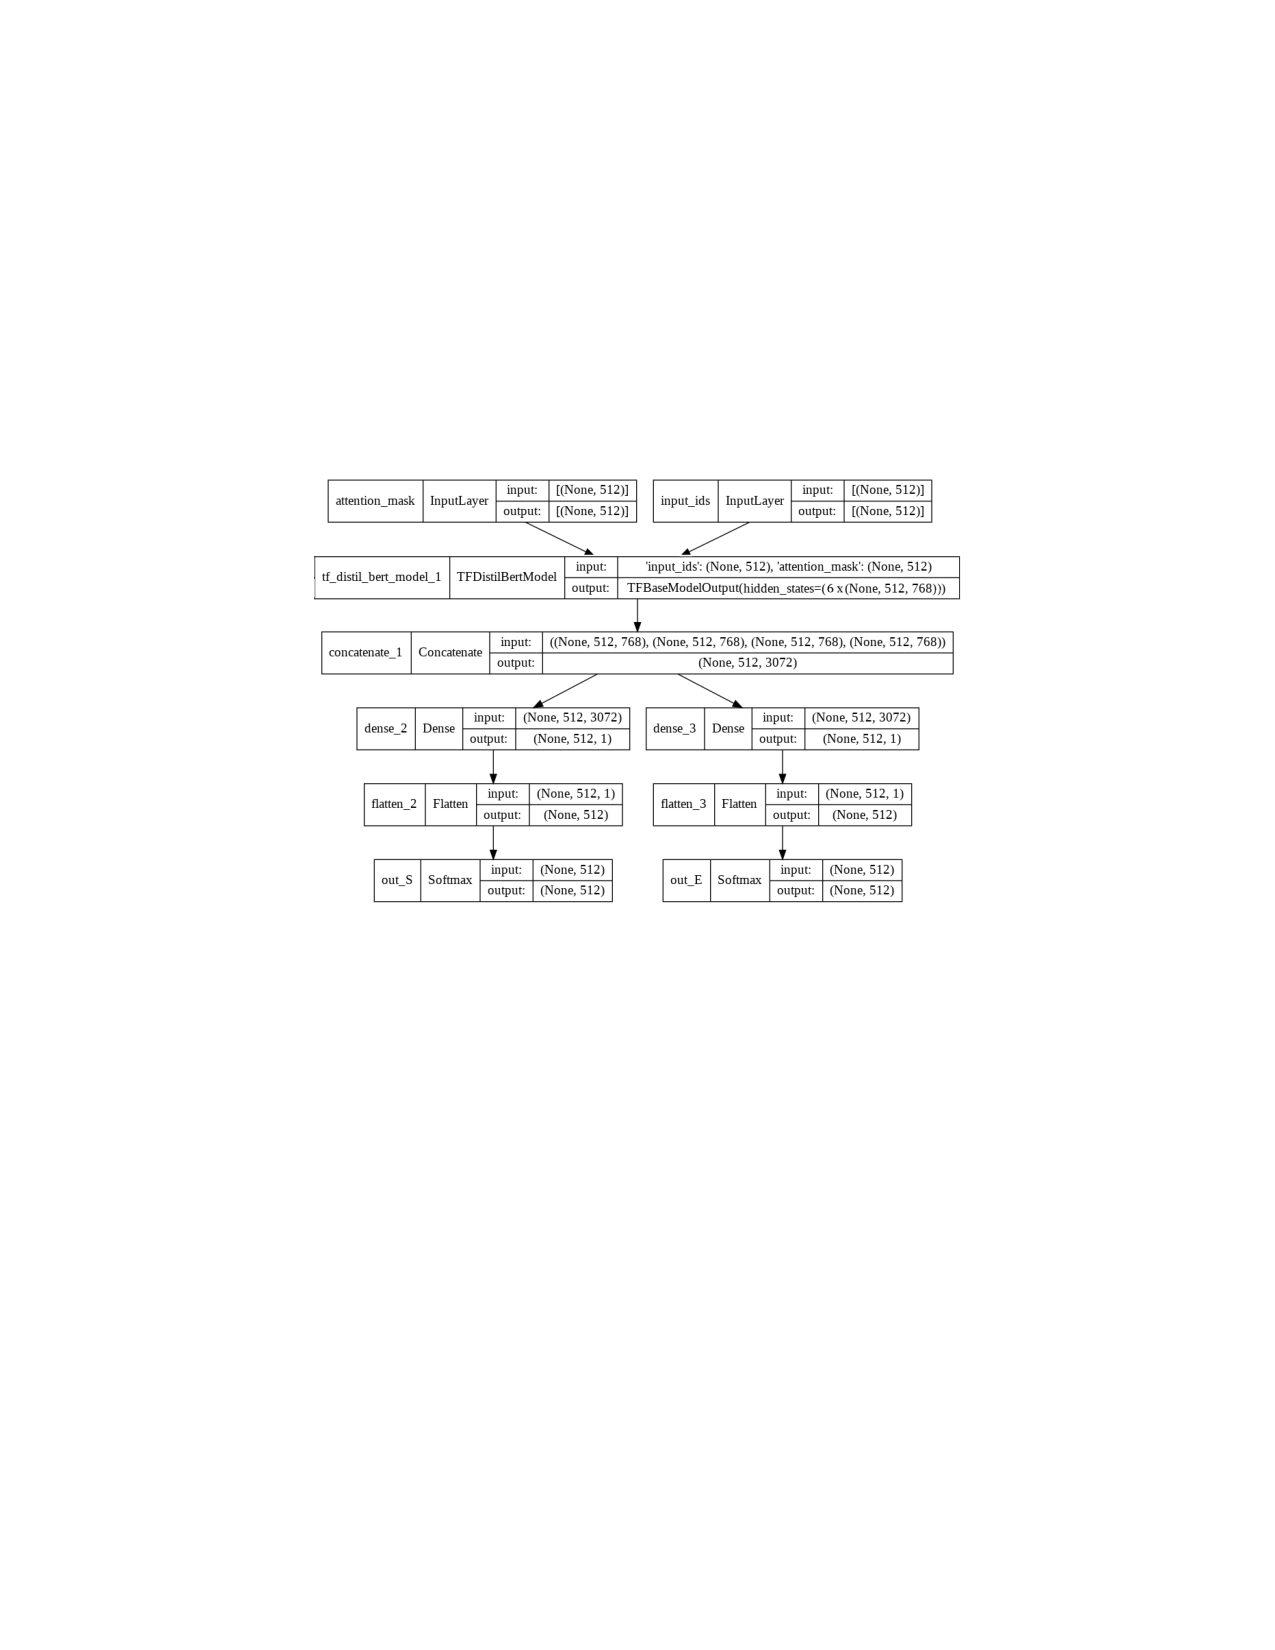
\includegraphics[width=\textwidth]{img/architecture.pdf}
    \caption{Model architecture}
    \label{fig:architecture}
\end{figure*}
}

\section{Approach}
\label{sec:system}
\attention{MAX 4 COLUMNS}

% write your system description here
\begin{figure*}[t]
    \centering
    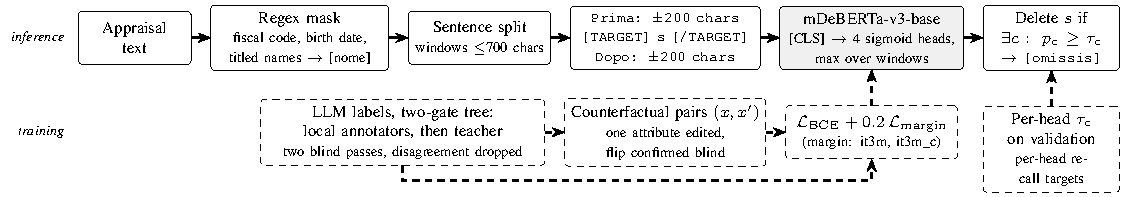
\includegraphics[width=\textwidth]{img/pipeline.pdf}
    \caption{Pipeline. The top row shows inference on one masked appraisal, while the bottom row (dashed) shows how labels, counterfactual pairs, the loss and the per-head thresholds are produced.}
    \label{fig:pipeline}
\end{figure*}

\paragraph{Task and formulation.} We evaluate every system on the same kind of decision, for each sentence $s$ and category $c$, it decides if the whole $s$ must be removed for $c$, and $s$ is replaced whole by \texttt{[omissis]} if any category fires. The systems differ only in what they see of the document, according to their specifications (Table~\ref{tab:systems}).

\begin{table}[t]
\centering\footnotesize
\setlength{\tabcolsep}{3pt}
\begin{tabular}{lp{0.2\columnwidth}p{0.48\columnwidth}}
\toprule
System & Sees & Fires for category $c$ when \\
\midrule
Presidio & sentence & any entity is found (category-agnostic) \\
GLiNER-PII & sentence & a span for label $c$ scores $\geq \tau_c$ \\
Gemma 12B & $\pm$2 sentences & its own decision (raw), or our policy applied to its answers (composed) \\
Students & $\pm$200 chars & head $c$ scores $\geq \tau_c$ \\
\bottomrule
\end{tabular}
\caption{What each system sees and how it decides. The masked text, the sentence segmentation, the deletion rule and the test sets are shared.}
\label{tab:systems}
\end{table}

\paragraph{Baselines.} We start by testing what is already available off the shelf, giving each system the input it was designed for. For \emph{Presidio} 2.2 we use spaCy \texttt{it\_core\_news\_lg} with the Italian recognisers, and we delete a sentence if any entity scores at least 0.5 (``any entity''). \emph{GLiNER-PII} (\texttt{gliner\_multi\_pii-v1}, the multilingual PII checkpoint of GLiNER) instead receives one natural-language label per category, for example ``health condition / disease / disability of a person''. A category $c$ fires if its best span reaches a per-category threshold $\tau_c$. We use it zero-shot, without fine-tuning, choosing English labels over Italian ones on validation, since the model is multilingual and covers Italian, but its labels work better in English (305 vs 221 of the 541 validation positives within the budget). Both Presidio and GLiNER-PII tag entities or spans in whatever text they receive, so they see the target sentence alone, since including neighbouring sentences might skew the judgement. As a small LLM we chose Gemma 4 12B instruct (4-bit, run locally). We prompt it with the teacher's own decision-tree prompt, giving it up to two sentences of context on each side, at temperature 0 with JSON output. We read its answer in two ways. \emph{Raw} takes its own final decision, while \emph{composed} ignores it and applies our two gates in code to its intermediate answers (topic, subject, living, assertion).

\paragraph{Student model.} As a student we chose mDeBERTa-v3-base (278M parameters). We fine-tuned it on the LLM labels, with a classification head on the \texttt{[CLS]} state and one sigmoid output per category $c$, plus a fifth ``other categories'' output inherited from early runs, which is never used for deletion. We encoded each sentence $s$ with its local context as \texttt{Prima: <200 chars> [TARGET] $s$ [/TARGET] Dopo: <200 chars>}, truncating to 384 tokens with the target kept whole (Figure~\ref{fig:pipeline}). The score $p_c$ is the maximum sigmoid output of head $c$ over the sentence's windows, and $s$ is removed if $p_c \geq \tau_c$ for any $c$. The loss is binary cross-entropy with per-head positive weights (the negative/positive ratio, capped at 10). All our following iterations share this architecture. The two gates are not built into the architecture, instead the model must learn them from the labels.

\paragraph{Counterfactual pairs.} In order to teach the gates rather than category words, we build a set of 741 real-derived counterfactual pairs from training groups only, the CF pairs. These pairs are built by editing one attribute of a real sentence while keeping the rest verbatim (e.g.\ ``A carico dell'esecutato risultano carichi pendenti'' becomes ``A carico dell'esecutato non risultano carichi pendenti''). Thus we end up with negation (207), hypothetical (145), deceased subject (27), company subject (13) and category swap (349) pairs. A fresh blind pass keeps only the pairs whose label flips as intended (agreement 94.9\%, $\kappa=0.898$). An original sentence and its twin always fall in the same micro-batch, and a check confirms zero overlap with every test set. The test twins (Table~\ref{tab:evalsets}) are built in the same way, from positives of documents that no model has seen (Appendix F).

\paragraph{Margin loss.} Binary cross-entropy scores the two members of a pair separately. Since an original and its twin share almost all their words, the model can keep BCE low by giving them similar scores and relying on category words, and in fact with BCE alone \texttt{it3} keeps only 3 of 54 negated twins. We therefore add a hinge that asks the original to score at least a margin $m$ above its twin, for the keep-type pairs $P$ (negated, hypothetical, deceased and company twins):
\begin{align*}
\ell(x,x')&=\tfrac{1}{|H_x|}\textstyle\sum_{c\in H_x}\bigl[m-z_c(x)+z_c(x')\bigr]_+\\
\mathcal{L}_{\mathrm{margin}}&=\tfrac{1}{|P|}\textstyle\sum_{(x,x')\in P}\ell(x,x')
\end{align*}
where $H_x$ are the heads positive for the original $x$, $z_c$ is the maximum logit of head $c$ over windows, $m=1$, and the total loss is $\mathcal{L}_{\mathrm{BCE}}+0.2\,\mathcal{L}_{\mathrm{margin}}$. We work on logits because near 1 the sigmoid flattens the gap, and category-swap pairs are excluded because both members must be removed.

\begin{table*}[t]
\centering\small
\setlength{\tabcolsep}{4.5pt}
\begin{tabular}{lcccccc}
\toprule
 & Held-out & IPW harmless & audit100 & Held-out doc & Cassazione & Negated twins \\
Model & recall (/372) & deletion (\%) & recall (/158) & leak (/116) & dec.\ leak (/307) & kept (/54) \\
\midrule
Presidio, any entity & 321 (86.3\%) & 52.87 & 122 (77.2\%) & 33 (28.4\%) & 77 (25.1\%) & -- \\
GLiNER-PII & 193 (51.9\%) & 11.49 & 68 (43.0\%) & 83 (71.6\%) & 141 (45.9\%) & -- \\
Gemma 4 12B, composed & 234 (62.9\%) & 0.00\textsuperscript{\S} & -- & 65 (56.0\%) & 158 (51.5\%) & -- \\
\midrule
\texttt{A0} & \textbf{371 (99.7\%)} & 7.25 & \textbf{157 (99.4\%)} & \textbf{1 (0.9\%)} & 13 (4.2\%) & 0 (0.0\%) \\
\texttt{it1}\textsuperscript{\dag} & 359 (96.5\%) & 2.29 & 156 (98.7\%) & 4 (3.4\%) & 69 (22.5\%) & 0 (0.0\%) \\
\texttt{it3} & \textbf{371 (99.7\%)} & \textbf{1.72} & 155 (98.1\%) & \textbf{1 (0.9\%)} & 22 (7.2\%) & 3 (5.6\%) \\
\texttt{it3m} & 369 (99.2\%) & 2.37 & 156 (98.7\%) & 3 (2.6\%) & 24 (7.8\%) & \textbf{39 (72.2\%)} \\
\texttt{it3m\_c} & \textbf{371 (99.7\%)} & 5.14 & \textbf{157 (99.4\%)} & \textbf{1 (0.9\%)} & \textbf{2 (0.7\%)} & 32 (59.3\%) \\
\bottomrule
\end{tabular}
\caption{Main results on the test sets. 95\% intervals for \texttt{A0} and \texttt{it3m\_c}: held-out recall 98.5--100\% (both), IPW deletion 6.56--8.05\% and 4.56--5.89\%, Cassazione leaks 2.5--7.1\% and 0.2--2.3\%. \textsuperscript{\dag}Single global threshold (0.060) chosen on audit100, so its audit100 values are optimistic. \textsuperscript{\S}On a weighted 600-sentence subsample, where \texttt{A0} gives 7.27\%. Baselines miss most originals, so their twins are omitted.}
\label{tab:main}
\end{table*}

\paragraph{Implementation.} All training and inference ran locally on one laptop (Apple M4 Max, 36 GB, PyTorch on MPS), using the encoder, Presidio, GLiNER and the LLM off the shelf through \texttt{transformers}, \texttt{presidio-analyzer} and \texttt{gliner}. Our contributions are the task formulation, the labelling policy, the counterfactual pair construction, pair-aware batching, the margin loss, the threshold rules and the evaluation design, while most of the code was written by AI coding agents under our direction (see the AI Report).

\explanation{
Describe the system or systems you have implemented (architectures, pipelines, etc.), and used to run your experiments. If you reuse parts of code written by others, be sure to make very clear your original contribution in terms of
\begin{itemize}
    \item architecture: is the architecture your design or did you take it from somewhere else
    \item coding: which parts of code are original or heavily adapted? adapted from existing sources? taken from external sources with minimal adaptations?
\end{itemize}
This also applies to AI-assisted coding.\\
It is a good idea to add figures to illustrate your pipeline and/or architecture(s)
(see Figure~\ref{fig:architecture})
}

\section{Experiments}
\label{sec:results}
\attention{MAX 3 COLUMNS}



% write your text here
\paragraph{\texttt{A0}.} We start by training \texttt{A0} on the 7,695 rows labelled by the two local annotators. We use AdamW (learning rate $2\cdot10^{-5}$, weight decay 0.01, 10\% linear warm-up), an effective batch of 32 and seed 42 for 5 epochs, and we keep the checkpoint with the lowest validation loss (epoch 4). These are standard fine-tuning values, fixed in advance and not tuned.

\paragraph{More teacher labels (\texttt{it1}).} \texttt{A0} deletes 7.25\% of harmless sentences, therefore we first try to make it more precise by adding harder real negatives. \texttt{it1} continues the training of \texttt{A0} for 500 updates (learning rate $10^{-5}$), where half of each batch replays A0-train, so that the model does not forget what it learned, while the other half comes from the Teacher rows, 1,132 real rows labelled by the teacher, and from the Edge suite, 1,157 synthetic sentences built from templates around the hard cases of the policy, such as negations and hypotheticals. Since the new rows follow the final policy, \texttt{it1} also shows what better labels alone can change. Differently from the other students, \texttt{it1} uses one global threshold on the maximum head score, chosen on audit100.

\paragraph{Counterfactual training (\texttt{it3}, \texttt{it3m}, \texttt{it3m\_c}).} Looking at the errors of \texttt{A0} (Section~\ref{sec:discussion}) we found the model exhibits signs of a shortcut, reacting to category words instead of applying the two gates. In order to fix it, \texttt{it3} continues \texttt{A0} for 800 updates (learning rate $10^{-5}$). Half of each batch is again replay, while the other half mixes the Edge suite (40\%), the CF pairs (35\%), the Teacher rows (15\%) and Cass-train, 500 Cassazione sentences rich in negations, taken from decisions that are not in the test set (10\%). These proportions were set by hand, giving most of the new half to the hard cases (Edge suite and CF pairs), and were not tuned. \texttt{it3m} is trained in the same way, with the margin loss on top (weight 0.2).

\paragraph{Threshold calibration.} For the systems that output a score per category, namely GLiNER-PII and our students, we choose one threshold $\tau_c$ per category on validation. Each category has a recall target (salute 0.95, penale 0.85, minori 0.98, famiglia 0.98), and for \texttt{A0} these targets give $\tau=(0.038, 0.407, 0.020, 0.072)$, which is \texttt{A0}'s ratified operating point. \texttt{it3} and \texttt{it3m} keep \texttt{A0}'s thresholds. However, the margin compresses the penale scores, therefore \texttt{it3m\_c} keeps the weights of \texttt{it3m} and only lowers $\tau_{\text{penale}}$ to 0.0098 (Appendix B). For GLiNER-PII we use the same targets, but we also require each category to fire on at most 5\% of the 899 all-negative validation rows, so among the thresholds that respect both we take the one with the highest precision, and if none reaches the target we take the one with the highest recall within this budget.

\paragraph{Metrics.} \emph{Recall} is the share of positive sentences removed by any head, reported with a 95\% confidence interval. A document \emph{leaks} if at least one of its positives is kept. To know whether a model deletes too much, we need harmless sentences that no model and no choice has ever touched, therefore we define \emph{harmless deletion} as the share of them that a model removes, measured on the 2,000 sentences of the IPW sample. These sentences are not drawn uniformly, so each one counts for as many sentences as it represents (details in Appendix E). Finally, to check whether two models really differ, we compare them on the same items and look only at the cases where one of them is right and the other is wrong, and if these cases are too unbalanced to be due to chance we consider the difference real.

\paragraph{Decision rule.} A variant replaces \texttt{A0} only if it has held-out recall $\geq 99\%$, audit100 recall $\geq 156/158$, no more held-out leaks than \texttt{A0} and a lower IPW deletion than \texttt{A0}. We fixed this rule before \texttt{it3m\_c}, but after seeing the results of \texttt{it3} and \texttt{it3m}.

\paragraph{Results.} Table~\ref{tab:main} reports all models on the five test sets. Looking at the baselines first, Presidio is the one reaching the highest recall, however this only happens because it deletes 52.87\% of the harmless sentences, so basically half of the text. GLiNER-PII, which we calibrated on validation in the same way as our students, reaches 51.9\% at 11.49\% harmless deletion, and none of its categories manages to reach the recall target while staying within the firing budget, while lowering a single threshold for all of them buys recall only with a massive deletion (95.7\% recall at 71.63\% deletion for $t=0.05$, Appendix C). Gemma, if we take its own decision, removes almost nothing (3.5\%), on the other hand composing its answers with our two gates raises the recall to 62.9\% with no harmless deletion in the subsample, although more than half of the held-out documents (65/116) still leak.

Our students are all far above the baselines. \texttt{A0} removes 371/372 held-out positives and 157/158 audit positives, paying for it with 7.25\% harmless deletion. \texttt{it1} trades recall for precision (96.5\% recall, 2.29\% deletion) and therefore fails the recall gate, and like \texttt{A0} it keeps none of the 54 negated twins, which means that adding labels from the teacher was not enough to remove the shortcut. \texttt{it3} is the one with the lowest deletion (1.72\%), but it misses three audit positives, leaks 22 Cassazione decisions and keeps only 3 negated twins, while adding the margin loss (\texttt{it3m}) brings the kept twins up to 39/54, at the price of the held-out leaks going up to 3/116. In the end \texttt{it3m\_c} is the only variant satisfying all four criteria, in fact it equals \texttt{A0} on held-out recall, audit recall and held-out leaks (each model leaks one document, a different one, $p=1.0$), and at the same time it deletes less harmless text (5.14\% vs 7.25\%), leaks fewer Cassazione decisions (2 vs 13, $p=0.0034$) and keeps 32/54 negated twins instead of none. If we look only at the keyword subset (115 positives), which is not biased by the model scores, \texttt{A0} and \texttt{it3m\_c} both reach 114/115, while Presidio gets 86.1\% and GLiNER-PII 50.4\%.

\explanation{
Describe how you set up your experiments: which architectures/configurations you used, which hyper-parameters and what methods used to set them, which optimizers, metrics, etc.
\\
Then, \textbf{use tables} to summarize your findings (numerical results) in validation and test. If you don't have experience with tables in \LaTeX, you might want to use \href{https://www.tablesgenerator.com/}{\LaTeX table generator} to quickly create a table template.
}

\section{Discussion}
\label{sec:discussion}
\attention{MAX 3 COLUMNS}

% write your analysis of the results here
\paragraph{Baseline errors.} All the baselines look for entities, while in our task what matters is the fact attached to a person, whose name is often already masked. Most of Presidio's hits are places, organisations and dates, but in appraisals addresses and dates are exactly the content we want to keep. GLiNER's labels instead behave lexically, in fact its minori head finds almost every minor (144/147 on validation), since a minor is usually a mention (``figlio minorenne''), while salute finds only 12 of 42, since an illness is a fact that can be expressed in many ways. Gemma fails in a different way, namely it usually reads the facts correctly but then it does not carry them through to the final decision, in fact on Cassazione almost all of its harmless removals (173 of 176) concern subjects that it had itself labelled as hypothetical. Composing the decision in code fixes part of this, but not enough.

\paragraph{Vocabulary shortcut.} We find that \texttt{A0}'s high recall does not mean that it learned the two gates. We found this by testing it on a keyword-mined frame of appraisals not used for training, where it deletes up to 40.2\% of the \emph{harmless} sentences containing salute, minori or penale keywords, against 7.5\% of those without, and on the twins, where it deletes all 54 negated and all 24 deceased-subject twins. Part of this comes from its labels, which were made before the negation and deceased rules existed, but even \texttt{it1}, which also sees labels that follow these rules, still keeps no negated twin. We suspect that much of the shortcut comes from the training data, since one third of A0-train is synthetic, so the keywords in it are easy to learn. On the other hand, synthetic data is what makes the rare heads work at all, since students trained only on real rows had to delete more than half of the harmless audit sentences to reach 156/158 recall.

\paragraph{Effect of the counterfactuals.} Adding the CF pairs to the training data was not enough on its own, since an original and its twin share almost all their words, so with BCE alone the model kept scoring them almost the same (\texttt{it3} kept only 3 of 54 negated twins). The margin term is what taught the model to look at the negation, because it penalises the difference between the two sentences rather than each score alone, while keeping in-domain recall above 99\% (39 of 54 negated twins kept). Deceased subjects instead did not change at all, probably because we had too few deceased pairs for the model to learn from. Finally, lowering the penale threshold is a trade-off, since \texttt{it3m\_c} recovers the Cassazione positives that \texttt{it3m} lost, but at the price of a few negated twins, which the penale head now removes too.

\paragraph{Error analysis.} Table~\ref{tab:errors} lists the main error types. Our final model fails mostly on abstract statements, namely sentences that talk about a crime or an illness in general, like statements of law or hypotheticals, without referring to a real person. This is probably due to the training data, since in appraisals a crime or an illness is almost always attached to someone, so the model never really had to check who the sentence is about. On Cassazione, where decisions discuss crimes and illnesses in the abstract, \texttt{it3m\_c} deletes 92.0\% of the harmless sentences with penale keywords (79.1\% for \texttt{A0}), and even in appraisals harmless sentences with keywords are deleted far more often than the others (up to 38.7\%, against 4.8\%). The margin therefore helped with negation, but it could not teach the model to check whether a keyword refers to a person, and for this adding abstract statements of law and hypotheticals to the training data would be the natural next step.

\begin{table}[t]
\centering\footnotesize
\setlength{\tabcolsep}{3pt}
\begin{tabular}{lp{0.37\columnwidth}l}
\toprule
Error type & Invented example & Who \\
\midrule
Keyword, no person & \emph{Il locale \`e adibito ad ambulatorio medico.} & \texttt{A0}, \texttt{it3m\_c} \\
Negated & \emph{Non risultano carichi pendenti a carico del debitore.} & \texttt{A0} (54/54) \\
Deceased & \emph{Il bene pervenne per successione dal padre, deceduto nel 2001.} & all (24/24) \\
Law statement & \emph{La legge prevede la sospensione della pena per grave malattia.} & \texttt{it3m\_c} \\
Masked party & \emph{L'esecutato \`e affetto da una grave invalidit\`a.} & baselines \\
\bottomrule
\end{tabular}
\caption{Error types with invented, anonymised examples. The first four are harmless sentences that get deleted (the law statement on Cassazione); the last is a positive that entity-based baselines keep.}
\label{tab:errors}
\end{table}

\begin{table}[t]
\centering\footnotesize
\begin{tabular}{lcc}
\toprule
Comparison & $\kappa$ & Exact match \\
\midrule
\multicolumn{3}{l}{\emph{119 sentences with both labels}} \\
Human vs teacher & 0.80 & 88.2\% \\
Human vs \texttt{A0}'s local annotators & 0.82 & 89.9\% \\
Teacher vs \texttt{A0}'s local annotators & 0.92 & 95.0\% \\
\midrule
\multicolumn{3}{l}{\emph{49 sentences from \texttt{A0}'s validation set}} \\
Human vs teacher & 0.69 & 79.6\% \\
Human vs \texttt{A0}'s local annotators & 0.41 & 30.6\% \\
\bottomrule
\end{tabular}
\caption{Human agreement with the LLM labels on 119 sentences with both a teacher label and an agreed label from \texttt{A0}'s local annotators (top), and on 49 sentences from \texttt{A0}'s old validation set, all marked sensitive by the local annotators (bottom). $\kappa$ is pooled over sentences and categories; exact match means the same categories.}
\label{tab:human}
\end{table}

\paragraph{Limitations.} (1) Every test reference is an LLM label, therefore one human annotator (the author) labelled 186 stratified sentences to check them. The human agrees with the teacher and with \texttt{A0}'s local annotators at a similar level, but on 49 sentences from \texttt{A0}'s old validation set much more with the teacher, since the local annotators over-flag rare categories (Table~\ref{tab:human}). (2) The in-domain evaluation is basically a famiglia result (369 of 372 held-out positives), and the claims on rare classes rest on Cassazione. (3) We chose \texttt{it3m\_c} among five variants after knowing their test results, since the shortcut could only be measured on the twins and on Cassazione, which have no validation counterpart. (4) Each model was trained once, with a single seed. (5) Every student starts from \texttt{A0} and replays A0-train, so \texttt{A0}'s older labels are part of every model, and a student trained from scratch on the final labels is left for future work.

\explanation{
Here you should make your analysis of the results you obtained in your experiments. Your discussion should be structured in two parts: 
\begin{itemize}
    \item discussion of quantitative results (based on the metrics you have identified earlier; compare with baselines);
    \item error analysis: show some examples of odd/wrong/unwanted outputs; reason about why you are getting those results, elaborate on what could/should be changed in future developments of this work. 
\end{itemize}
You don't need to copy the examples here if they're too long to fit: you can refer to the notebook, or use the Appendix at the end of the report.
}

\section{Conclusion}
\label{sec:conclusion}
\attention{MAX 1 COLUMN}

% write your conclusions here
In this work we tried to remove sensitive sentences from Italian expert appraisals with a small model that runs on a laptop, distilling into an mDeBERTa encoder a two-gate policy applied by LLM annotators. Our final model removes 371 of 372 held-out positives while deleting about 5\% of the harmless sentences, which is far beyond what entity-based tools and a zero-shot 12B LLM can do, and with 279M parameters it processes about 45 sentences per second, while a 12B LLM is 150 to 529 times slower (Appendix D). The most interesting result for us was however a negative one, since a near-perfect in-domain recall was hiding a model that ignored negation and the living-person gate, and we only noticed it thanks to the counterfactual twins and the Supreme Court decisions. Counterfactual pairs alone did not fix this, while a margin loss on them taught the model to keep most negated twins. With one lowered threshold, our final model then leaks far fewer Cassazione decisions than \texttt{A0} at the same in-domain recall, although out of domain it still deletes too many abstract statements.

The main limitations are the small human check and the post-hoc model selection (Section~\ref{sec:discussion}), so as next steps we would like to add a second annotator, more deceased and hypothetical pairs and several seeds.

\explanation{
In one or two paragraphs, recap your work and main results.
What did you observe? 
Did all go according to expectations? 
Was there anything surprising or worthwhile mentioning?
After that, discuss the main limitations of the solution you have implemented, and indicate promising directions for future improvement.
}

\aireport

% write your AI report here
AI was used in two different roles.

\paragraph{AI as part of the method.} LLMs produced all the reference labels, as described in Sections~\ref{sec:data} and~\ref{sec:system}. Two local open models (Qwen3.6-27B, Gemma 4 12B) labelled \texttt{A0}'s training data, and local LLMs wrote its synthetic rows. We used GPT-6.1 Sol as the teacher for all later labels, the counterfactual edits and the Cassazione labels. Hosted LLMs labelled and quality-checked audit100. Gemma 4 12B is also one of our baselines. We treat these outputs as data produced by models, not as human judgements.

\paragraph{AI assistance.} AI coding agents (Claude Code and Codex) wrote most of the experiment code and ran most of the experiments under my direction. I defined the task, the labelling policy and its rulings, the evaluation design and every go/no-go decision. Claude drafted the teacher prompt from my written rulings, and the root-cause review of the failed retrains was carried out with both agents, before I ratified the resulting plan. During my manual validation the assistant explained the guideline on request and walked through 2 example items, which I excluded from the metrics. All numbers come from one canonical results file, regenerated by a script from aggregate outputs. AI was also used to polish the language of the report.

\bibliography{nlpreport.bib}

% comment the following line if you don't have external links
\externallinks

% list your external links here
\begin{itemize}\itemsep0pt
\item Code (including all prompts and the mask rules) and aggregate result files: \url{https://github.com/klein-t/sensitive-sentence-removal-it}. The corpus contains personal data and is not released.
\item mDeBERTa-v3-base: \url{https://huggingface.co/microsoft/mdeberta-v3-base}
\item GLiNER-PII: \url{https://huggingface.co/urchade/gliner_multi_pii-v1}
\item Gemma 4 12B (run locally as a 4-bit MLX conversion): \url{https://huggingface.co/google/gemma-4-12B-it}
\item Presidio: \url{https://github.com/microsoft/presidio}
\item Portale delle Vendite Pubbliche (public judicial sale listings): \url{https://pvp.giustizia.it}
\item Corte di Cassazione public decisions: \url{https://www.italgiure.giustizia.it/sncass/}
\end{itemize}

% comment the following line if you don't have an appendix
\myappendix

% write your appendix here
\subsection*{A. Policy rules and their legal basis}
Table~\ref{tab:policy} shows which rules of our policy follow from the law and which ones are our own design choices, with all citations referring to Regulation (EU) 2016/679 \citep{gdpr} and to D.Lgs.~196/2003 as amended \citep{codiceprivacy}.

\begin{table}[t]
\centering\footnotesize
\setlength{\tabcolsep}{4pt}
\begin{tabular}{lll}
\toprule
Rule & Basis & Status \\
\midrule
salute & art.~9(1) & law \\
penale & art.~10; C.~2-octies & law \\
minori & C.~52(5); rec.~38 & analogy \\
famiglia & C.~52(5) & analogy \\
Masked party: identifiable & rec.~26 & law \\
Hypothetical: keep & no subject & law \\
Deceased: keep & rec.~27 & law\textsuperscript{*} \\
Negated: keep & art.~10 (arguably) & choice \\
Company seizure: remove & rec.~14 & choice \\
\bottomrule
\end{tabular}
\caption{Which policy rules follow from the law and which are our design choices (art.\ and rec.\ are GDPR articles and recitals, C.\ are Codice privacy articles). minori and famiglia are not art.~9 categories; art.~52 covers judicial decisions and is applied by analogy. \textsuperscript{*}The exception for an implicated living heir is our choice.}
\label{tab:policy}
\end{table}

\subsection*{B. Thresholds and validation}
\texttt{A0}'s thresholds for salute, penale, minori and famiglia are 0.0384, 0.40721, 0.02048 and 0.07239, and \texttt{it3m\_c} keeps them except for penale, which we lowered to 0.0098325, since the margin compresses the penale scores and at \texttt{A0}'s threshold the penale head of \texttt{it3m} almost never fires. Table~\ref{tab:val} shows how the two models behave on validation.

\begin{table}[t]
\centering\footnotesize
\begin{tabular}{lcc}
\toprule
Head & \texttt{A0} & \texttt{it3m\_c} \\
\midrule
salute & 6, 40/42 & 4, 35/42 \\
penale & 16, 46/53 & 43, 49/53 \\
minori & 3, 146/147 & 6, 145/147 \\
famiglia & 39, 293/299 & 28, 287/299 \\
\bottomrule
\end{tabular}
\caption{Negatives fired (of 899) and recall on validation.}
\label{tab:val}
\end{table}

\subsection*{C. Per-class results and GLiNER-PII}
Both \texttt{A0} and \texttt{it3m\_c} remove every rare held-out positive, and on Cassazione \texttt{it3m\_c} misses only two positives. GLiNER-PII instead cannot reach any recall target within the 5\% budget, and a single global threshold does not help either, since it buys recall only with a massive deletion (95.7\% recall at 71.63\% deletion with $t=0.05$).

\subsection*{D. Speed and size}
We measured the speed of each system end to end on 20 test documents, always on the same laptop (Table~\ref{tab:speed}). \texttt{it3m\_c} is about as fast as GLiNER-PII, Presidio is faster, and the 12B LLM is 150 to 529 times slower.

\begin{table}[t]
\centering\footnotesize
\setlength{\tabcolsep}{3pt}
\begin{tabular}{lllrr}
\toprule
System & Size & Device & Sent./s & ms/sent. \\
\midrule
\texttt{it3m\_c} & 279M & GPU & 45.5 & 22 \\
GLiNER-PII & 289M & GPU & 42.7 & 23 \\
Presidio & rules+CNN & CPU & 295.8 & 3 \\
Gemma 12B & 12B, 4-bit & GPU & 0.09--0.3 & 3.3k--11.6k \\
\bottomrule
\end{tabular}
\caption{Size and speed of each system on one laptop (Apple M4 Max, 36 GB).}
\label{tab:speed}
\end{table}

\subsection*{E. Harmless-deletion estimate}
We split the 56,094 sentences of the IPW documents into seven bands by the highest score of \texttt{A0} and \texttt{it1}, and drew about 286 sentences per band, so that the rare uncertain sentences are well represented. Each sampled sentence then counts for as many sentences as it represents in its band, so harmless deletion becomes
{
\begin{equation}
\hat{D}=\frac{\sum_{i\in H} w_i\,\mathbf{1}[\text{$i$ deleted}]}{\sum_{i\in H} w_i},\qquad w_i=\frac{N_{b(i)}}{n_{b(i)}},
\end{equation}}
where $H$ is the set of sampled harmless sentences, $b(i)$ the band of sentence $i$, and $N_b$ and $n_b$ the sizes of band $b$ in all the documents and in the sample. This is the standard Horvitz-Thompson estimator \citep{horvitz1952generalization}, and since the weights depend only on how we sampled, it holds for any model.

\subsection*{F. Test sets in detail}
\emph{Held-out.} We looked for candidates in two rounds, in 338 documents drawn from the 868 that no model and no choice has ever used. In each round we took random sentences containing keywords, plus the 150 keyword sentences that \texttt{A0} and \texttt{it1} scored highest, and we labelled all of them with two teacher passes. Since the score-mined part, which gives 257 of the 372 positives, favours these two models, we also report the 115 positives found by keywords only, namely the keyword subset.

\emph{IPW sample.} See Appendix E.

\emph{Audit100.} We reserved 100 test documents and had them labelled sentence by sentence by hosted LLMs, then a larger LLM checked blind the sentences that contain a keyword or were flagged ($\kappa=0.862$). Since this check only read these sentences, a positive missed by both labellers cannot be recovered.

\emph{Cassazione.} We took public civil and criminal decisions of the Italian Supreme Court from 2021 to 2026 (see the Links section), found their sentences by keywords only, at most three per decision, and labelled them with two teacher passes, which agree on 98.4\% of them ($\kappa=0.964$). None of these decisions is in Cass-train.

\emph{Twins.} Starting from real positives of unseen documents, the teacher edits one attribute (negation, deceased subject, company subject or category), leaving the context and the OCR noise as they are, and then a fresh blind pass keeps only the pairs whose label flips as intended.

\end{document}